\section{Git Branches}
\begin{frame}[fragile]
  \slidetitle

  In this section, we will learn how to:
  \begin{itemize}
    \item Create and delete a branches
    \item Work with branches
    \item Rebase branches
    \item Merge branches
  \end{itemize}
\end{frame}

\subsection{The master branch}
\begin{frame}[fragile]
  \subslidetitle

  With git, you are always working on a branch and the default git branch is called \cmd{master}.

\end{frame}

\subsection{Creating branches}
\begin{frame}[fragile]
  \subslidetitle

  To create a new \cmd{foo} branch, append the branch name to the \cmd{git branch} command:
  \begin{lstlisting}
(*\textcolor[HTML]{18B2B2}{(master)}*) $ (*\textcolor[HTML]{0000AA}{git branch foo}*)
\end{lstlisting}

  The \cmd{git branch} command lists you all your local branches:
  \begin{lstlisting}
(*\textcolor[HTML]{18B2B2}{(master)}*) $ (*\textcolor[HTML]{0000AA}{git branch}*)
  foo
* (*\textcolor[HTML]{00AA00}{master}*)
\end{lstlisting}

Note: The branch you are currently on is marked with an asterisk (*).
\end{frame}

\subsection{Switching to branch}
\begin{frame}[fragile]
  \subslidetitle
  The \cmd{git checkout} command, is used to change the working branch:
  \begin{lstlisting}
(*\textcolor[HTML]{18B2B2}{(master)}*) $ (*\textcolor[HTML]{0000AA}{git checkout foo}*)
Switched to branch 'foo'
(*\textcolor[HTML]{18B2B2}{(foo)}*) $ (*\textcolor[HTML]{0000AA}{git branch}*)
* (*\textcolor[HTML]{00AA00}{foo}*)
  master
\end{lstlisting}

  The \cmd{git checkout} command with \cmd{-b} option creates a new branch and automatically switch to it:
  \begin{lstlisting}
(*\textcolor[HTML]{18B2B2}{(foo)}*) $ (*\textcolor[HTML]{0000AA}{git checkout -b bar}*)
Switched to a new branch 'bar'
(*\textcolor[HTML]{18B2B2}{(bar)}*) $ (*\textcolor[HTML]{0000AA}{git branch}*)
* (*\textcolor[HTML]{00AA00}{bar}*)
  foo
  master
\end{lstlisting}
\end{frame}

\subsection{Deleting a branch}
\begin{frame}[fragile]
  \subslidetitle
  To delete an existing branch use the \cmd{-d} or \cmd{-D} (force) flag:
\begin{lstlisting}
(*\textcolor[HTML]{18B2B2}{(bar)}*) $ (*\textcolor[HTML]{0000AA}{git checkout master}*)
(*\textcolor[HTML]{18B2B2}{(master)}*) $ (*\textcolor[HTML]{0000AA}{git branch foo bar -d}*)
Deleted branch foo (was c974445).
Deleted branch bar (was 9adadac).
(*\textcolor[HTML]{18B2B2}{(master)}*) $ (*\textcolor[HTML]{0000AA}{git branch}*)
* (*\textcolor[HTML]{00AA00}{master}*)
\end{lstlisting}

  Note: you cannot delete the branch you are currently working on.
\end{frame}

% in general use diff to instruct changes

% create bugfix branch
\subsection{bugfix}
\begin{frame}[fragile]
    \subslidetitle

  Our first bug report was filled out:
  \newline \vspace{1em}
  \#1: The title of the html page does not match the backgound.

  Start to create a new bugfix branch and implement the fix:
  \begin{lstlisting}
(*\textcolor[HTML]{18B2B2}{(master)}*) $ (*\textcolor[HTML]{0000AA}{git checkout -b fix-title}*)
\end{lstlisting}

  Modify the moon.html file following this diff instructions:
  \begin{lstlisting}
diff --git a/moon.html b/moon.html
index 145cfff..ae7bc15 100644
--- a/moon.html
+++ b/moon.html
(*\textcolor[HTML]{18B2B2}{@@ -7,7 +7,8 @@}*)
         <style>
             body {
                 font-family: Monospace;
(*\textcolor{red}{-}*)                (*\textcolor{red}{background-color: \#f0f0f0; <!-- grey -->}*)
(*\textcolor[HTML]{00AA00}{+}*)                (*\textcolor[HTML]{00EE00}{background-color: black;}*)
(*\textcolor[HTML]{00AA00}{+}*)                (*\textcolor[HTML]{00EE00}{color: white;}*)
                 margin: 0px;
                 overflow: hidden;
             }
\end{lstlisting}
\end{frame}

% git diff master branch
\subsection{Display difference between branches}
\begin{frame}[fragile]
  \subslidetitle

  As git has the complete history locally, we can easily display changes between branches:

  \begin{lstlisting}
  (*\textcolor[HTML]{18B2B2}{(fix-title)}*) $ (*\textcolor[HTML]{0000AA}{git diff master}*)
  diff --git a/moon.html b/moon.html
  index 145cfff..ae7bc15 100644
  --- a/moon.html
  +++ b/moon.html
  (*\textcolor[HTML]{18B2B2}{@@ -7,7 +7,8 @@}*)
           <style>
               body {
                   font-family: Monospace;
  (*\textcolor{red}{-}*)                (*\textcolor{red}{background-color: \#f0f0f0; <!-- grey -->}*)
  (*\textcolor[HTML]{00AA00}{+}*)                (*\textcolor[HTML]{00EE00}{background-color: black;}*)
  (*\textcolor[HTML]{00AA00}{+}*)                (*\textcolor[HTML]{00EE00}{color: white;}*)
                   margin: 0px;
                   overflow: hidden;
               }
\end{lstlisting}
\end{frame}

% make a change on master
\subsection{Another change on the master}
\begin{frame}[fragile]
  \subslidetitle

  In the meantime, we need to update the README file with a Prerequisites sub-section:
  \begin{lstlisting}
(*\textcolor[HTML]{18B2B2}{(fix-title)}*) $ (*\textcolor[HTML]{0000AA}{git checkout master}*)
(*\textcolor[HTML]{18B2B2}{(master)}*) $ (*\textcolor[HTML]{0000AA}{echo "}*)
> (*\textcolor[HTML]{0000AA}{\#\# Prerequisites >> README"}*)
(*\textcolor[HTML]{18B2B2}{(master)}*) $ (*\textcolor[HTML]{0000AA}{git commit -a -m "add the prerequisites subsection"}*)
\end{lstlisting}

\end{frame}

% display with tig/gitk

\subsection{Graphic display in tig}
\begin{frame}[fragile]
  \subslidetitle

  Now we can see the graphical representation of our fix-title branch with \cmd{tig}:
  \begin{lstlisting}
  (*\textcolor[HTML]{18B2B2}{(master)}*) $ (*\textcolor[HTML]{0000AA}{tig master fix-title}*)
\end{lstlisting}

  \vspace{1em}

  \centerline{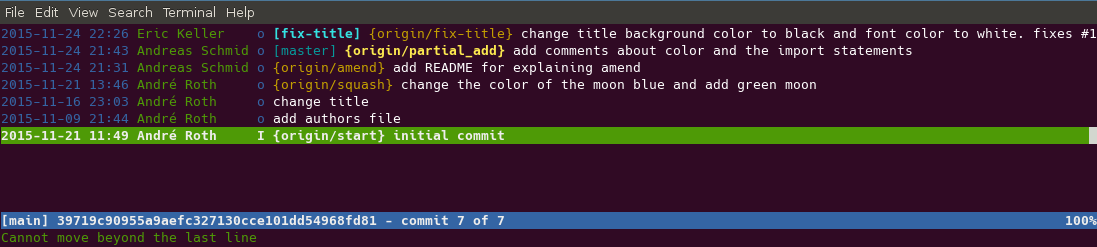
\includegraphics[width=10.5cm]{../screen/tig-fix-title.png}}

\end{frame}

\subsection{Graphic display in gitk}
\begin{frame}[fragile]
  \subslidetitle

  Now we can see the graphical representation of our fix-title branch with \cmd{gitk}:
  \begin{lstlisting}
  (*\textcolor[HTML]{18B2B2}{(master)}*) $ (*\textcolor[HTML]{0000AA}{gitk}*)
\end{lstlisting}

  \vspace{1em}

  \centerline{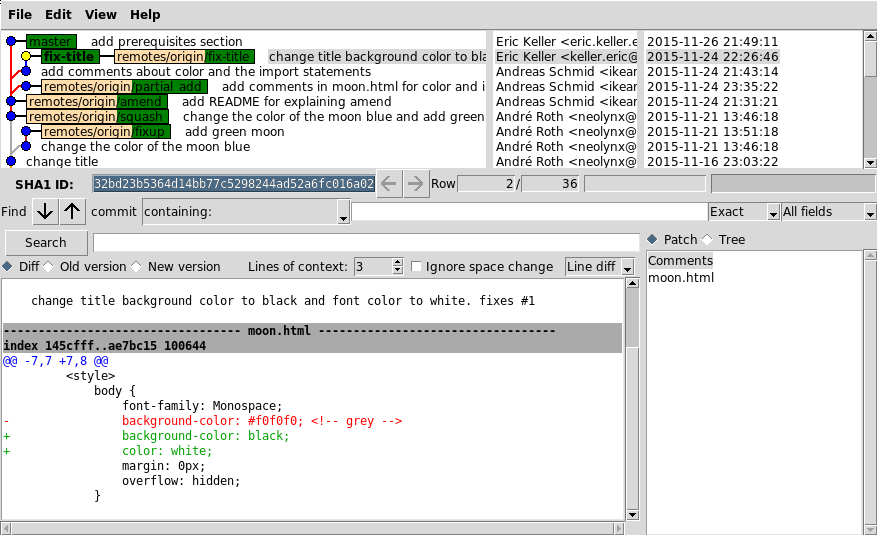
\includegraphics[width=10cm]{../screen/gitk-fix-title.png}}

\end{frame}

% rebase with master
\subsection{Rebasing a branch on top of master}
\begin{frame}[fragile]
  \subslidetitle

  Use \cmd{git rebase} to update the status of a branch on top of another branch:

  \begin{lstlisting}
(*\textcolor[HTML]{18B2B2}{(master)}*) $ (*\textcolor[HTML]{0000AA}{git checkout fix-title}*)
(*\textcolor[HTML]{18B2B2}{(fix-title)}*) $ (*\textcolor[HTML]{0000AA}{git rebase master}*)
First, rewinding head to replay your work on top of it...
Applying: add comments about color and the import statements
Applying: change title background color to black and font color to white. fixes #1
\end{lstlisting}

  As git states the rebase re-apply commits from the fix-title branches on to of the master branch.

\end{frame}

% display with tig/gitk
\subsection{Display rebase operation}
\begin{frame}[fragile]
  \subslidetitle

  Now we can see the graphical representation of our fix-title branch rebased on the master branch with \cmd{tig}:
  \begin{lstlisting}
(*\textcolor[HTML]{18B2B2}{(fix-title)}*) $ (*\textcolor[HTML]{0000AA}{tig master fix-title}*)
\end{lstlisting}

  \vspace{1em}

  \centerline{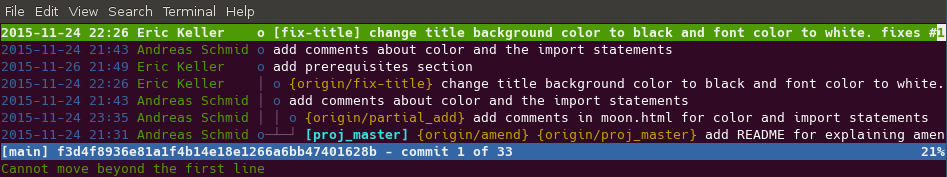
\includegraphics[width=10cm]{../screen/tig-fix-title-rebase-master.png}}

\end{frame}
% create another feature branch

\subsection{Create a feature branch}
\begin{frame}[fragile]
  \subslidetitle

  A new feature request has to be implemented on from the master branch:
  \newline \vspace{1em}
  \#2 insert a white moon between the blue and green moon.
  \begin{lstlisting}
(*\textcolor[HTML]{18B2B2}{(fix-title)}*) $ (*\textcolor[HTML]{0000AA}{git checkout -b feature-flag-color master}*)
Switched to a new branch 'feature-flag-color'
\end{lstlisting}
  Modify the moon.js file following this diff instructions:
  \begin{lstlisting}
diff --git a/moon.js b/moon.js
index 69d1726..b45cf20 100644
--- a/moon.js
+++ b/moon.js
(*\textcolor[HTML]{18B2B2}{@@ -3,6 +3,7 @@}*) var moons = [];
 
 init();
 moon( "blue" );
(*\textcolor[HTML]{00AA00}{+}*)(*\textcolor[HTML]{00AA00}{moon( "white" );}*)
 moon( "green" );
 animate();
\end{lstlisting}
  Commit your changes:
  \begin{lstlisting}
(*\textcolor[HTML]{18B2B2}{(fix-title)}*) $ (*\textcolor[HTML]{0000AA}{git commit -a -m "add a white moon between the blue and green moon, implements \#2"}*)
\end{lstlisting}

\end{frame}


\subsection{Some urgent change on master}
\begin{frame}[fragile]
  \subslidetitle

  An emergency fix has to be done on the master branch:
  \newline \vspace{1em}
  \#3 In our moon requirement, we never specified any green moon, modify it asap to red:
  \begin{lstlisting}
(*\textcolor[HTML]{18B2B2}{(fix-title)}*) $ (*\textcolor[HTML]{0000AA}{git checkout master}*)
Switched to branch 'master'
Your branch is up-to-date with 'origin/master'.
\end{lstlisting}
  Modify the moon.js file following this diff instructions:
  \begin{lstlisting}
diff --git a/moon.js b/moon.js
index 69d1726..9d851a7 100644
--- a/moon.js
+++ b/moon.js
(*\textcolor[HTML]{18B2B2}{@@ -3,7 +3,7 @@}*) var moons = [];
 
 init();
 moon( "blue" );
(*\textcolor{red}{-}*)(*\textcolor{red}{moon( "green" );}*)
(*\textcolor[HTML]{00AA00}{+}*)(*\textcolor[HTML]{00AA00}{moon( "red" );}*)
 animate();
\end{lstlisting}

  Commit your changes:
  \begin{lstlisting}
(*\textcolor[HTML]{18B2B2}{(fix-title)}*) $ (*\textcolor[HTML]{0000AA}{git commit -a -m "change green moon to red, fixes \#3"}*)
\end{lstlisting}

\end{frame}
% 2 commits on this branch
% display with tig/gitk
% merge with master branch
% display with tig/gitk


% git checkout branch which was edited a long time ago, and we can continue to edit at this stage.


\subsection{git stash}
\begin{frame}[fragile]
    \subslidetitle
% clean, pop,
\end{frame}

\subsection{git diff}
\begin{frame}[fragile]
    \subslidetitle
\end{frame}

\subsection{Rebase a branch}
\begin{frame}[fragile]
    \subslidetitle
% -i
\end{frame}

\subsection{Merge a branch}
\begin{frame}[fragile]
    \subslidetitle
\end{frame}

\subsection{Rebase vs. Merge}
\begin{frame}[fragile]
    \subslidetitle
\end{frame}

\subsection{Cherrypick a commit}
\begin{frame}[fragile]
    \subslidetitle
\end{frame}

